\documentclass[margin=1in]{article}
\usepackage[utf8]{inputenc}
\usepackage[english]{babel}
\usepackage{amsmath}
\usepackage{graphicx}
\usepackage{capt-of}
\usepackage{lipsum}
\usepackage{graphicx}
\usepackage{caption}
\usepackage{subcaption}
\usepackage{listings}
\usepackage{hyperref} 
\usepackage{xcolor} % For custom colors
\lstset{
	language=Python,                % Choose the language (e.g., Python, C, R)
	basicstyle=\ttfamily\small, % Font size and type
	keywordstyle=\color{blue},  % Keywords color
	commentstyle=\color{gray},  % Comments color
	stringstyle=\color{red},    % String color
	numbers=left,               % Line numbers
	numberstyle=\tiny\color{gray}, % Line number style
	stepnumber=1,               % Numbering step
	breaklines=true,            % Auto line break
	backgroundcolor=\color{black!5}, % Light gray background
	frame=single,               % Frame around the code
}
\usepackage{float}
\usepackage[margin=1in]{geometry}
\usepackage[]{amsthm} %lets us use \begin{proof}
	\usepackage[]{amssymb} %gives us the character \varnothing
	

	
	\title{Homework 2, IEOR 4732}
	\author{Zongyi Liu}
	\date{Feb 11, 2025}
	\begin{document}
		\maketitle
		
		\subsection*{Question 1}
		 The characteristic function of the log of stock price in Black-Scholes framework is given by:
		$$
		\begin{aligned}
			\mathbb{E}\left(e^{i u \ln S_t}\right) & =\mathbb{E}\left(e^{i u s_t}\right) \\
			& =\exp \left(i\left(\ln S_0+\left(r-q-\frac{\sigma^2}{2}\right) t\right) u-\frac{1}{2} \sigma^2 u^2 t\right) \\
			& =\exp \left(i\left(s_0+\left(r-q-\frac{\sigma^2}{2}\right) t\right) u-\frac{1}{2} \sigma^2 u^2 t\right)
		\end{aligned}
		$$
		
		For the following parameters:
		Spot price, $S_0=\$ 1900$; maturity, $T=0.25$ year; volatility, $\sigma=0.36$; risk-free interest rate, $r=2.00 \%$, continuous dividend rate, $q=1.87 \%$ and strike range of $K=2000,2100,2200$ price European call options via the following transform techniques:
		
		\begin{itemize}
		\item 	(a) Fast Fourier transform (FFT): consider $\eta=\Delta \nu=0.25, \alpha=0.4,1.0,1.4,3.0, N=2^n$ for $n=9,11,13,15$, and $\beta=\ln K-\frac{\lambda N}{2}$
		\item 	(b) Fractional fast Fourier transform (FrFFT): consider $\eta=\Delta \nu=0.25, \lambda=\Delta k=0.1, \alpha=0.4,1.0,1.4,3.0, N=2^n$ for $n=6,7,8,9$, and $\beta=\ln K-\frac{\lambda N}{2}$
		\item 	(c) Fourier-cosine (COS) method: consider values $[-1,1],[-4,4],[-8,8],[-12,12]$ for the interval $[a, b]$ and find the sensitivity of your results to the choice of $[a, b]$
		\end{itemize}
		
		Compare and conclude.

	\textbf{Answer}
	
	  \subsubsection*{Part a}
	  
	  I modified the code given in the \texttt{sample code} folder, and get the result of Fast Fourier transform for different strike prices.
	 \begin{table}[h!]
	 	\centering
	 	\caption{Results for Different Values of $K$}
	 	\scalebox{0.84}{ % Adjust 0.8 to your desired scale
	 		\begin{tabular}{|c|c|c|c|c||c|c|c|c||c|c|c|c|}
	 			\hline
	 			& \multicolumn{4}{c||}{$K=2000,\ \eta =0.25$} & \multicolumn{4}{c||}{$K=2100,\ \eta =0.25$} & \multicolumn{4}{c|}{$K=2200,\ \eta =0.25$} \\
	 			\hline
	 			$\alpha$ & $N=2^9$ & $2^{11}$ & $2^{13}$ & $2^{15}$ & $N=2^9$ & $2^{11}$ & $2^{13}$ & $2^{15}$ & $N=2^9$ & $2^{11}$ & $2^{13}$ & $2^{15}$ \\
	 			\hline
	 			0.4 & 95.3281 & 95.3281 & 95.3281 & 95.3281 & 64.9160 & 64.9160 & 64.9160 & 64.9160 & 43.0286 & 43.0286 & 43.0286 & 43.0286 \\
	 			\hline
	 			1.0 & 95.2467 & 95.2467 & 95.2467 & 95.2467 & 64.8346 & 64.8346 & 64.8346 & 64.8346 & 42.9472 & 42.9472 & 42.9472 & 42.9472 \\
	 			\hline
	 			1.4 & 95.2467 & 95.2467 & 95.2467 & 95.2467 & 64.8346 & 64.8346 & 64.8346 & 64.8346 & 42.9472 & 42.9472 & 42.9472 & 42.9472 \\
	 			\hline
	 			3.0 & 95.2467 & 95.2467 & 95.2467 & 95.2467 & 64.8346 & 64.8346 & 64.8346 & 64.8346 & 42.9472 & 42.9472 & 42.9472 & 42.9472 \\
	 			\hline
	 	\end{tabular}}
	 \end{table}
	 

\subsubsection*{Part b}

The fractional FFT procedure computes a sum of the form
$$
\sum_{\gamma=1}^{N} e^{-i 2 \pi \gamma(j-1)(m-1)} x(j)
$$
for any value of $\gamma$
   I modified the sample codes given, which only contains methods for \texttt{VG}, \texttt{GBM}, and \texttt{Heston}.
   
   I added the chunk like:
   
   \begin{lstlisting}
   	elif model == 'BlackScholes':  
   	sigma = 0.36  # Volatility  
   	params.append(sigma)  
   \end{lstlisting}
   
   and in \texttt{def generic CF}, define the model:
   
   \begin{lstlisting}
   	elif (model == 'BlackScholes'):
   	sigma = params[0]  # Volatility
   	
   	mu = np.log(S0) + (r - q - 0.5 * sigma**2) * T  # Drift
   	a = sigma * np.sqrt(T)  
   	phi = np.exp(1j * mu * u - 0.5 * a**2 * u**2) 
   \end{lstlisting} 

   Which defines the Black-Scholes model, and we can get the result for different of strike price. 


 \begin{table}[h!]
	\centering
	\caption{Results for Different Values of $K$}
	\scalebox{0.84}{ % Adjust 0.8 to your desired scale
		\begin{tabular}{|c|c|c|c|c||c|c|c|c||c|c|c|c|}
			\hline
			& \multicolumn{4}{c||}{$K=2000,\ \eta =0.25$} & \multicolumn{4}{c||}{$K=2100,\ \eta =0.25$} & \multicolumn{4}{c|}{$K=2200,\ \eta =0.25$} \\
			\hline
			$\alpha$ & $N=2^6$ & $2^{7}$ & $2^{8}$ & $2^{9}$ & $N=2^6$ & $2^{7}$ & $2^{8}$ & $2^{9}$ & $N=2^6$ & $2^{7}$ & $2^{8}$ & $2^{9}$ \\
			\hline
			0.4 & 95.3859 & 95.3295 & 95.3295 & 95.3295 &64.9425 & 64.9174 &  64.9174 &  64.9174 & 43.0108 & 43.0298 & 43.0298 & 43.0298  \\
			\hline
			1.0 & 95.3051 & 95.2477 & 95.2477 & 95.2477& 64.8774  & 64.8357 & 64.8357 & 64.8357 & 42.9511 & 42.9482 & 42.9482 & 42.9482 \\
			\hline
			1.4 & 95.3006& 95.2475 & 95.2475 & 95.2475 & 64.8842 & 64.8355 & 64.8355 & 64.8355 & 42.9641 & 42.9480 & 42.9480 & 42.9480 \\
			\hline
			3.0 & 95.2521 & 95.2467 & 95.2467 & 95.2467 & 64.8762 & 64.8349 & 64.8349 & 64.8349 & 42.9915 & 42.9476 & 42.9476 & 42.9476 \\
			\hline
	\end{tabular}}
\end{table}
	  

	  The FrFFT analyzes a signal at non-integer frequency intervals, whereas the FFT simply calculates the standard frequency spectrum of a discrete signal with increased speed.
	  
	  \subsubsection*{Part c}
	  
	  The Fourier cosine series expansion of a function $f(\theta)$ on $[0, \pi]$ is
	  $$
	  \begin{aligned}
	  	f(\theta) & =\frac{1}{2} A_{0}+\sum_{k=1}^{\infty} A_{k} \cos \left(k_{k}^{s} \theta\right) \\
	  	& =\sum_{\substack{i n}}^{\infty}{ }_{k=0}^{\infty} A_{k} \cos (k \theta)
	  \end{aligned}
	  $$
	  with the Fourier cosine coefficient
	  $$
	  A_{k}=\frac{2}{\pi} \int_{0}^{\pi} f(\theta) \cos (k \theta) d \theta
	  $$
	  where $\bar{\sum}$ indicates the first term in the summation is weighted by one-half.
	  
	  Then the option value at time $t$ can be written as
	  
	  $$
	  \begin{aligned}
	   & v(x, t)=C \int_{a}^{b} v(y, T) f(y \mid x)^{0} d y \\
	  	& =C \int_{a}^{b b^{25}} v(y, T) \bar{\sum}_{k=0}^{\infty} A_{k} \cos \left(k \frac{y-a}{b-a} \pi\right) d y \\
	  	& =C \sum_{k=0}^{\infty} A_{k}\left(\int_{a}^{b} v(y, T) \cos \left(k \frac{y-a}{b-a} \pi\right) d y\right)
	  \end{aligned}
	  $$
	
	Here I tested different values for the interval $[a,b]$, and results are different. 
	\begin{table}[h!]
		\centering
		\begin{tabular}{|c|c|c|c|c|}
			\hline
			\multicolumn{5}{|c|}{Fourier-Cosine Method} \\
			\hline
			$K$ & $[-1,1]$  & $[-4,4]$ & $[-8,8]$ & $[-12,12]$  \\
			\hline
			2000 &2994.5770 & 4965.5228  & 4975.0742 & 4975.2406\\
			\hline
			2100 & 3144.3059 & 5213.7990 & 5223.8279 & 5224.0026 \\
			\hline
			2200 & 3294.0347 & 5462.0751 & 5472.5816 & 5472.7646 \\
			\hline
		\end{tabular}
	\end{table}

And the result can be plotted below:

\begin{figure}[h]
	\caption{Sensitivity of Option Prices to Interval [a,b]}
	\centering
	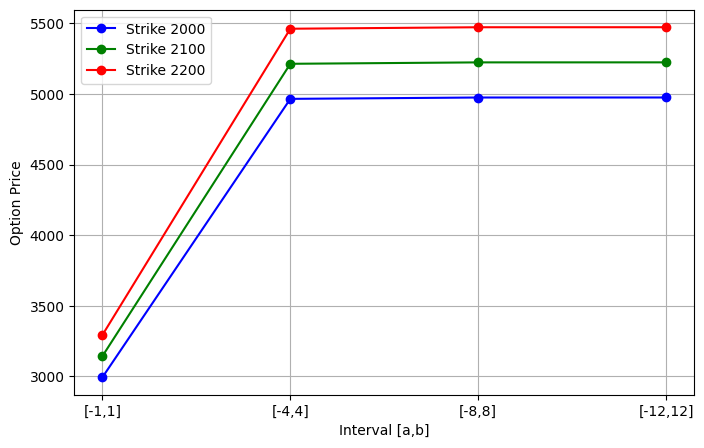
\includegraphics[width=0.7\textwidth]{HW1_Q3}
\end{figure}

% Shows "Example Website"
 I later looked up in Fang and Oosterlee's \href{http://ta.twi.tudelft.nl/mf/users/oosterle/oosterlee/COS.pdf}{paper}, they proposed some rule of thumb based on cumulants to get an idea how to choose $[a, b]$. In particular, they suggested (In equation (49)):
$$
[a, b]= \begin{cases}{\left[c_1 \pm 12 \sqrt{c_2}\right]} & , n_c=2 \\ {\left[c_1 \pm 10 \sqrt{c_2+\sqrt{c_4}}\right]} & , n_c=4 \\ {\left[c_1 \pm 10 \sqrt{c_2+\sqrt{c_4+\sqrt{c_6}}}\right]} & , n_c=6\end{cases}
$$
where $c_1, c_2, c_4, c_6$ are the first, second, forth and sixth cumulants of $\ln \left(S_t / K\right)$. The cumulants, $c_n$, are defined by the cumulant-generating function $g(t)$ :
$$
g(t)=\log \left(E\left(e^{t \cdot X}\right)\right)
$$

for some random variable $X$. The cumulants are given by the derivatives, at zero, of $g(t)$. Back to our model, when $L$ is chosen as 8, which corresponds to $[-4,4]$, the premiums are more accurate and consistent.


	\clearpage
	
	\subsection*{Appendix}
\subsubsection*{Part a}
	\begin{lstlisting}
	import numpy as np
	import math
	import time
	import cmath
	
	# Fixed Parameters
	S0 = 1900  # Initial stock price
	K = 2000    # Strike price
	k = math.log(K)  # Log of strike price
	r = 0.02  # Risk-free rate
	q = 0.0187  # Dividend yield
	T = 0.25     # Time to maturity
	
	# Parameters for FFT 
	n = 15     # n determines the size of FFT: N = 2^n
	N = 2**n
	eta = 0.25 # Step-size
	alpha = 1.0 # Damping factor
	
	# Black-Scholes model parameters
	sigma = 0.36  # Volatility
	
	# Characteristic function for Black-Scholes
	def generic_CF(u, S0, r, q, T, sigma):
	mu = np.log(S0) + (r - q - 0.5 * sigma**2) * T
	a = sigma * np.sqrt(T)
	phi = np.exp(1j * u * mu - 0.5 * a**2 * u**2)
	return phi
	
	# FFT implementation for Black-Scholes model
	def genericFFT(S0, K, r, q, T, alpha, eta, n, sigma):
	N = 2**n
	lda = (2 * np.pi / N) / eta  # Step-size in log strike space
	beta = np.log(K)
	
	# Initialize arrays
	km = np.zeros(N)
	xX = np.zeros(N, dtype=complex)
	
	# Discount factor
	df = np.exp(-r * T)
	
	# Define the frequency range
	nuJ = np.arange(N) * eta
	psi_nuJ = generic_CF(nuJ - (alpha + 1) * 1j, S0, r, q, T, sigma) / ((alpha + 1j * nuJ) * (alpha + 1 + 1j * nuJ))
	
	# Compute the xX vector (values for the FFT)
	for j in range(N):
	km[j] = beta + j * lda
	wJ = eta if j > 0 else eta / 2  # Weighting for j = 0
	xX[j] = np.exp(-1j * beta * nuJ[j]) * df * psi_nuJ[j] * wJ
	
	# Apply FFT to the xX vector
	yY = np.fft.fft(xX)
	
	# Compute the option prices
	cT_km = np.zeros(N)
	for i in range(N):
	multiplier = np.exp(-alpha * km[i]) / np.pi
	cT_km[i] = multiplier * np.real(yY[i])
	
	return km, cT_km
	
	# Function to calculate option price using FFT
	def calculate_option_price(S0, K, r, q, T, alpha, eta, n, sigma):
	start_time = time.time()
	
	km, cT_km = genericFFT(S0, K, r, q, T, alpha, eta, n, sigma)
	cT_k = np.interp(k, km, cT_km)  # Interpolating the option price for the given strike
	
	elapsed_time = time.time() - start_time
	print(f"Option via FFT: for strike {np.exp(k):.4f} the option premium is {cT_k:.4f}")
	print(f"FFT execution time was {elapsed_time:.7f} seconds")
	
	return cT_k
	
	# Example usage
	option_price = calculate_option_price(S0, K, r, q, T, alpha, eta, n, sigma)
	\end{lstlisting}

\subsubsection*{Part b}
       \begin{lstlisting}
       	
       	import warnings
       	warnings.filterwarnings("ignore")
       	
       	import numpy as np
       	import cmath
       	import math
       	import time
       	
       	# Fixed Parameters
       	S0 = 1900
       	K = 2100
       	k = math.log(K)
       	r = 0.02
       	q = 0.0187
       	
       	# Parameters for FFT and FrFFT 
       	
       	n_FFT = 7
       	N_FFT = 2**n_FFT
       	
       	n_FrFFT = 7
       	N_FrFFT = 2**n_FrFFT
       	
       	N = 2000
       	
       	#step-size
       	eta = 0.25
       	# damping factor
       	alpha = 3
       	
       	# step-size in log strike space
       	lda_FFT = (2*math.pi/N_FFT)/eta # lda is fixed under FFT
       	lda_FrFFT = 0.001 # lda is an adjustable parameter under FrFFT, 
       	
       	
       	#Choice of beta
       	beta = np.log(S0)-N*lda_FFT/2
       	#beta = np.log(S0)-N*lda_FrFFT/2
       	#beta = np.log(K)
       	
       	#model-specific Parameters
       	model = 'BlackScholes'
       	
       	params = []     
       	if (model == 'GBM'):
       	
       	sig = 0.30
       	params.append(sig);
       	
       	elif model == 'BlackScholes':  
       	sigma = 0.36  # Volatility  
       	params.append(sigma)  
       	
       	elif (model == 'VG'):
       	
       	sig = 0.3
       	nu = 0.5
       	theta = -0.4
       	#
       	params.append(sig);
       	params.append(nu);
       	params.append(theta);
       	
       	
       	
       	elif (model == 'Heston'):
       	
       	kappa = 2.0
       	theta = 0.05
       	sig = 0.30
       	rho = -0.70
       	v0 = 0.04
       	#
       	params.append(kappa)
       	params.append(theta)
       	params.append(sig)
       	params.append(rho)
       	params.append(v0)
       	
       	def generic_CF(u, params, S0, r, q, T, model):
       	
       	if (model == 'GBM'):
       	
       	sig = params[0]
       	mu = np.log(S0) + (r-q-sig**2/2)*T
       	a = sig*np.sqrt(T)
       	phi = np.exp(1j*mu*u-(a*u)**2/2)
       	
       	elif (model == 'BlackScholes'):
       	sigma = params[0]  # Volatility
       	
       	mu = np.log(S0) + (r - q - 0.5 * sigma**2) * T  # Drift
       	a = sigma * np.sqrt(T)  # Standard deviation over the maturity period
       	phi = np.exp(1j * mu * u - 0.5 * a**2 * u**2)  # Characteristic function for Black-Scholes
       	
       	
       	elif(model == 'Heston'):
       	
       	kappa  = params[0]
       	theta  = params[1]
       	sigma  = params[2]
       	rho    = params[3]
       	v0     = params[4]
       	
       	tmp = (kappa-1j*rho*sigma*u)
       	g = np.sqrt((sigma**2)*(u**2+1j*u)+tmp**2)
       	
       	pow1 = 2*kappa*theta/(sigma**2)
       	
       	numer1 = (kappa*theta*T*tmp)/(sigma**2) + 1j*u*T*r + 1j*u*math.log(S0)
       	log_denum1 = pow1 * np.log(np.cosh(g*T/2)+(tmp/g)*np.sinh(g*T/2))
       	tmp2 = ((u*u+1j*u)*v0)/(g/np.tanh(g*T/2)+tmp)
       	log_phi = numer1 - log_denum1 - tmp2
       	phi = np.exp(log_phi)
       	
       	#g = np.sqrt((kappa-1j*rho*sigma*u)**2+(u*u+1j*u)*sigma*sigma)
       	#beta = kappa-rho*sigma*1j*u
       	#tmp = g*T/2
       	
       	#temp1 = 1j*(np.log(S0)+(r-q)*T)*u + kappa*theta*T*beta/(sigma*sigma)
       	#temp2 = -(u*u+1j*u)*v0/(g/np.tanh(tmp)+beta)
       	#temp3 = (2*kappa*theta/(sigma*sigma))*np.log(np.cosh(tmp)+(beta/g)*np.sinh(tmp))
       	
       	#phi = np.exp(temp1+temp2-temp3);
       	
       	
       	elif (model == 'VG'):
       	
       	sigma  = params[0];
       	nu     = params[1];
       	theta  = params[2];
       	
       	if (nu == 0):
       	mu = np.log(S0) + (r-q - theta -0.5*sigma**2)*T
       	phi  = np.exp(1j*u*mu) * np.exp((1j*theta*u-0.5*sigma**2*u**2)*T)
       	else:
       	mu  = np.log(S0) + (r-q + np.log(1-theta*nu-0.5*sigma**2*nu)/nu)*T
       	phi = np.exp(1j*u*mu)*((1-1j*nu*theta*u+0.5*nu*sigma**2*u**2)**(-T/nu))
       	
       	return phi
       	def evaluateIntegral(params, S0, K, r, q, T, alpha, eta, N, model):
       	
       	# Just one strike at a time
       	# no need for Fast Fourier Transform
       	
       	# discount factor
       	df = math.exp(-r*T)
       	
       	sum1 = 0
       	for j in range(N):
       	nuJ = j*eta
       	psi_nuJ = df*generic_CF(nuJ-(alpha+1)*1j, params, S0, r, q, T, model)/((alpha + 1j*nuJ)*(alpha+1+1j*nuJ))
       	if j == 0:
       	wJ = (eta/2)
       	else:
       	wJ = eta
       	sum1 += np.exp(-1j*nuJ*k)*psi_nuJ*wJ
       	
       	cT_k = (np.exp(-alpha*k)/math.pi)*sum1
       	
       	return np.real(cT_k) 
       	
       	def genericFFT(params, S0, K, r, q, T, alpha, eta, n, model):
       	
       	N = 2**n
       	
       	# step-size in log strike space
       	lda = (2*np.pi/N)/eta
       	
       	#Choice of beta
       	#beta = np.log(S0)-N*lda/2
       	#beta = np.log(K)
       	
       	# forming vector x and strikes km for m=1,...,N
       	km = np.zeros((N))
       	xX = np.zeros((N))
       	
       	# discount factor
       	df = math.exp(-r*T)
       	
       	nuJ = np.arange(N)*eta
       	psi_nuJ = generic_CF(nuJ-(alpha+1)*1j, params, S0, r, q, T, model)/((alpha + 1j*nuJ)*(alpha+1+1j*nuJ))
       	
       	for j in range(N):  
       	km[j] = beta+j*lda
       	if j == 0:
       	wJ = (eta/2)
       	else:
       	wJ = eta
       	
       	xX[j] = np.exp(-1j*beta*nuJ[j])*df*psi_nuJ[j]*wJ
       	
       	yY = np.fft.fft(xX)
       	cT_km = np.zeros((N))  
       	for i in range(N):
       	multiplier = np.exp(-alpha*km[i])/math.pi
       	cT_km[i] = multiplier*np.real(yY[i])
       	
       	return km, cT_km
       	
       	def genericFrFFT(params, S0, K, r, q, T, alpha, eta, n, lda, model):
       	
       	N = 2**n
       	gamma = eta*lda/(2*math.pi)
       	
       	#Choice of beta
       	#beta = np.log(S0)-N*lda/2
       	beta = np.log(K)
       	
       	# initialize x, y, z, and cT_km
       	km = np.zeros((N))
       	x = np.zeros((N))
       	y = np.zeros((2*N), dtype=np.complex128)
       	z = np.zeros((2*N), dtype=np.complex128)
       	cT_km = np.zeros((N)) 
       	
       	# discount factor
       	df = math.exp(-r*T)
       	
       	# compute x
       	nuJ = np.arange(N)*eta
       	psi_nuJ = generic_CF(nuJ-(alpha+1)*1j, params, S0, r, q, T, model)/((alpha + 1j*nuJ)*(alpha+1+1j*nuJ))
       	
       	for j in range(N):  
       	km[j] = beta+j*lda
       	if j == 0:
       	wJ = (eta/2)
       	else:
       	wJ = eta
       	x[j] = np.exp(-1j*beta*nuJ[j])*df*psi_nuJ[j]*wJ
       	
       	# set up y
       	for i in range(N):
       	y[i] = np.exp(-1j*math.pi*gamma*i**2)*x[i]
       	y[N:] = 0
       	
       	# set up z
       	for i in range(N):
       	z[i] = np.exp(1j*math.pi*gamma*i**2)
       	z[N:] = z[:N][::-1]
       	
       	# compute xi_hat
       	xi_hat = np.fft.ifft(np.fft.fft(y) * np.fft.fft(z))
       	
       	# compute call prices
       	for i in range(N):
       	cT_km[i] = np.exp(-alpha*(beta + i*lda))/math.pi * (np.exp(-1j*math.pi*gamma*i**2)*xi_hat[i]).real
       	
       	return km, cT_km
       	
       	print(' ')
       	print('===================')
       	print('Model is %s' % model)
       	print('-------------------')
       	
       	T = 0.25
       	
       	# FFT
       	print(' ')
       	start_time = time.time()
       	km, cT_km = genericFFT(params, S0, K, r, q, T, alpha, eta, n_FFT, model)
       	#cT_k = cT_km[0]
       	cT_k = np.interp(k, km, cT_km)
       	
       	elapsed_time = time.time() - start_time
       	
       	#cT_k = np.interp(np.log(k), km, cT_km)
       	print("Option via FFT: for strike %s the option premium is %6.4f" % (np.exp(k), cT_k))
       	#print("Option via FFT: for strike %s the option premium is %6.4f" % (np.exp(k), cT_km[0]))
       	print('FFT execution time was %0.7f' % elapsed_time)
       	
       	# FrFFT
       	print(' ')
       	start_time = time.time()
       	km, cT_km = genericFrFFT(params, S0, K, r, q, T, alpha, eta, n_FrFFT, lda_FrFFT, model)
       	#cT_k = cT_km[0]
       	cT_k = np.interp(k, km, cT_km)
       	
       	elapsed_time = time.time() - start_time
       	
       	#cT_k = np.interp(np.log(), km, cT_km)
       	print("Option via FrFFT: for strike %s the option premium is %6.4f" % (np.exp(k), cT_k))
       	#print("Option via FFT: for strike %s the option premium is %6.4f" % (np.exp(k), cT_km[0]))
       	print('FrFFT execution time was %0.7f' % elapsed_time)
       	
       	
       	# Integral
       	print(' ')
       	start_time = time.time()
       	cT_k = evaluateIntegral(params, S0, K, r, q, T, alpha, eta, N, model)
       	elapsed_time = time.time() - start_time
       	print("Option via Integration: for strike %s the option premium is %6.4f" % (np.exp(k), cT_k))
       	print('Evaluation of integral time was %0.7f' % elapsed_time)
       	
       	 \end{lstlisting}
	
\subsubsection*{Part c}
   
		 \begin{lstlisting}
		
   	    
   	        import numpy as np
   	        def char_func(u, S0, r, q, sigma, T):
   	        """ Black-Scholes characteristic function """
   	        return np.exp(1j * u * (np.log(S0) + (r - q - 0.5 * sigma**2) * T) - 0.5 * sigma**2 * u**2 * T)
   	        
   	        def cos_method_call(S0, K, T, r, q, sigma, N, a, b):
   	        """ Fourier-Cosine method for European call option pricing """
   	        x0 = np.log(S0 / K)
   	        
   	        # Compute coefficients
   	        k = np.arange(N)
   	        omega_k = k * np.pi / (b - a)
   	        
   	        # Characteristic function evaluations
   	        phi_k = char_func(omega_k, S0, r, q, sigma, T) * np.exp(-1j * omega_k * a)
   	        
   	        # Payoff function coefficients
   	        chi_k = (np.sin(omega_k * (b - a)) - np.sin(omega_k * (-a))) / omega_k
   	        chi_k[0] = b - a  # Handle k=0 separately
   	        
   	        # COS method summation
   	        V = np.real(phi_k * chi_k * 2 / (b - a))
   	        
   	        # Discounted expectation
   	        call_price = np.exp(-r * T) * np.sum(V)
   	        return call_price * K
   	        
   	        # Parameters
   	        S0 = 1900  # Spot price
   	        T = 0.25  # Maturity in years
   	        sigma = 0.36  # Volatility
   	        r = 0.02  # Risk-free rate
   	        q = 0.0187  # Continuous dividend rate
   	        strike_prices = [2000, 2100, 2200]  # Strike prices
   	        N = 100  # Number of terms in Fourier series
   	        intervals = [(-1, 1), (-4, 4), (-8, 8), (-12, 12)]  # Intervals [a, b]
   	        
   	        # Compute option prices for different intervals
   	        results = {}
   	        for a, b in intervals:
   	        results[(a, b)] = {K: cos_method_call(S0, K, T, r, q, sigma, N, a, b) for K in strike_prices}
   	        
   	        # Print results
   	        for (a, b), prices in results.items():
   	        print(f"Interval [{a}, {b}]:")
   	        for K, price in prices.items():
   	        print(f"  Strike {K}: {price:.4f}")
   	    
   \end{lstlisting}
		
    
	\end{document}